\documentclass[conference,10pt,a4paper]{IEEEtran}
\usepackage{times}
\usepackage{graphicx}
\usepackage{booktabs}
\usepackage{amsmath}
\usepackage{amssymb}
\usepackage{url}
\usepackage[hidelinks]{hyperref}
\usepackage{caption}
\captionsetup{justification=raggedright,singlelinecheck=false}
\usepackage{algorithm}
\usepackage{algpseudocode}
\usepackage{placeins}

\begin{document}
\raggedbottom

\title{Seasonal-Lag and Multi-Track Ensembling for Drought Severity Forecasting (DM~114 Kaggle)}

\author{
\IEEEauthorblockN{Team 3 --- Yu-Shun Liu (413551030), Tung-Hao Chang (413551038), Kuan-Fu Chen (414551017)}
\IEEEauthorblockA{
Data Mining, Spring 2026\\
NYCU\\
\url{https://github.com/RaisoLiu/dm-114-final-project}
}
}

\maketitle

\begin{abstract}
This paper presents the reported final solution of \textbf{Team 3} for the DM~114 (Spring 2026) Final Project Kaggle competition: predicting five future weekly drought severity scores (integer $0$--$5$) from 91 days of regional meteorological history. The Kaggle metric is the mean absolute error (MAE), and the public repository is \url{https://github.com/RaisoLiu/dm-114-final-project}.

The submission blends a six-leg gradient-boosted decision tree (GBDT) anchor over two feature families (b91, pl), an autoregressive seasonal-lag lookup at a $\approx$6-year period (2215 d), a weather-only dilated 1-D CNN, and an SSL-pretrained Transformer; weights ($A{=}0.20$, $B{=}0.45$, $C{=}0.25$, $D{=}0.10$) come from a single training menu and are followed by a public-slice affine-and-clip calibration. The selected submission achieves a public-leaderboard MAE of \textbf{0.7628}, a 10.6\% relative reduction over the prior team ceiling of $0.8534$. Section~\ref{sec:ortho} reports the iter4 recomputed per-region residual correlations of each non-GBDT leg with the GBDT anchor (lag-2215: $\rho{=}0.51$ with 95\% CI $[0.485, 0.533]$; CNN: $\rho{=}0.54$; SSL: $\rho{=}0.33$, lowest), and Table~\ref{tab:t5} is the controlled OOF-aligned 9-row ablation that decomposes the method components. The artefact is regenerated as a cached re-blend by \texttt{make phd-below075}, byte-verified against the archived CSV by \texttt{make verify-submission}; the cross-leg correlations and the 9-row ablation are reproduced by \texttt{make ablation}.
\end{abstract}

\section{Project Summary}

\subsection{Task}
For each of $R=2{,}248$ regions, the training table \texttt{train.csv} provides 5{,}480 consecutive days of daily meteorological observations (16 features such as precipitation, temperature, humidity, wind, surface pressure) and a weekly United States Drought Monitor (USDM)-style severity score in $\{0,1,2,3,4,5\}$ that is non-null on exactly one day of every 7. The test table \texttt{test.csv} provides, for the \emph{same} 2{,}248 regions, an additional 91-day weather-only window starting from each region's last training day. The objective is to predict, for each region, the scores at the next 5 weekly anchors after the 91-day input window (\texttt{pred\_week1}\,\ldots\,\texttt{pred\_week5}). The official metric is MAE, lower is better.

\subsection{Why random splits fail}
Random train/validation splits are invalid here. Within a region the score series exhibits strong autocorrelation (mean per-region lag-7 autocorrelation $> 0.7$) and a dominant multi-year periodic component (Section~\ref{sec:periodicity}), so a randomly held-out anchor sees its own immediate future leak through the training set. All experiments therefore use a \emph{time-based, leakage-safe} validation split that respects the 91-day input window and the public-leaderboard slice's position within the 6-year drought cycle.

\subsection{High-level method}
After fifteen structurally distinct attempts hit the same empirical ceiling, we identified two complementary signal families: (i) an autoregressive seasonal-lag baseline at $2215$\,d --- using only the provided historical training labels in \texttt{train.csv}, with no test labels, no external labels, and no external data --- targeting the $\approx$6-year cycle, and (ii) weather-only deep models (a dilated 1-D CNN and an SSL-pretrained Transformer) trained without score input. The training menu's premise that lag-2215 was the most orthogonal signal (originally estimated at $\rho\approx 0.107$ in a 5-fold region-CV that did not preserve aligned per-row predictions) was re-audited in iter4 with regenerated aligned OOF predictions: the SSL Transformer is now the least-correlated leg with the GBDT anchor ($\rho{=}0.33$), while lag-2215 and CNN sit around $\rho{\approx}0.5$ (Section~\ref{sec:ortho}). Family diversity, rather than a single ultra-low-$\rho$ leg, drives the blend gain. Blending these legs with the anchor under a public-slice affine-and-clip calibration produces the final $0.7628$ public-MAE artefact, captured in one JSON ``training menu'' and reproduced by \texttt{make phd-below075}.

\section{Related Work}

Time-series tabular forecasting on multi-region, multi-feature panels is most commonly tackled with gradient-boosted decision trees (GBDT) such as LightGBM~\cite{ke2017lightgbm} and HistGradientBoosting, which excel on heterogeneous numerical features and missing values. For pure sequence modelling, WaveNet-style dilated causal convolutions~\cite{vandenoord2016wavenet} have proven effective in Kaggle forecasting competitions, including sales forecasting~\cite{kechyn2018wavenet} that is itself referenced by the DM~114 assignment. Pre-trained foundation models for time series, notably \emph{Chronos}~\cite{ansari2024chronos}, enable zero-shot and few-shot transfer to new domains. For multi-horizon forecasting with interpretable attention, Lim et al.\ introduced the Temporal Fusion Transformer~\cite{lim2021tft}.

In the drought domain specifically, the US Drought Monitor (USDM)~\cite{svoboda2002usdm} provides the canonical weekly $0$--$5$ severity labels that the competition simulates. Validation and confidence-interval estimation in this paper follow Efron's bootstrap~\cite{efron1979bootstrap}.

Our work is closest in spirit to the WaveNet+GBDT ensembles of \cite{kechyn2018wavenet}, but the key methodological novelty is the explicit use of a seasonal autoregressive component aligned with the observed multi-year periodicity, rather than only adding another learned model.

\section{Proposed Method}
\label{sec:method}

\subsection{Notation and problem formulation}
Let $x_{r,t}\in\mathbb{R}^{16}$ denote the 16 daily weather features for region $r$ on day $t$. A 91-day input window ending on a valid score day $t$ is $X_{r,t}=(x_{r,t-90},\ldots,x_{r,t})$. The 5 weekly targets are $y_{r,t}^{(h)}=\mathrm{score}_{r,t+7h}$ for $h\in\{1,\ldots,5\}$. The training loss for a single horizon $h$ is the mean absolute error
\[
\mathcal{L}_h(\hat f) = \tfrac{1}{|\mathcal D|}\sum_{(r,t)\in\mathcal D}\bigl|\hat f(X_{r,t}) - y_{r,t}^{(h)}\bigr|,
\]
where $\mathcal D$ contains every $(r,t)$ such that all five targets $y_{r,t}^{(1\ldots 5)}$ are non-null. Final predictions are clipped to $[0,5]$ to match the valid label range.

\subsection{Leakage-safe window construction}
Algorithm~\ref{alg:windows} produces the supervised training tensor used by every model. It matches the windowing format of \texttt{test.csv} (91 days of weather followed by 5 weekly score requests, never seeing future scores); the public-like validation slice additionally matches the median cutoff-age of $\approx$531 days between the last training label and the prediction window.

\begin{algorithm}
\caption{Leakage-safe 91-day window construction}
\label{alg:windows}
\begin{algorithmic}[1]
\For{each region $r$}
  \For{each anchor day $t$ with score$(r,t)\neq\mathrm{NaN}$}
    \State $X \gets$ weather rows $[t{-}90, t]$ for region $r$
    \State $y \gets [\mathrm{score}(r,t{+}7h)]_{h=1}^{5}$
    \If{any $y_h$ is NaN} \State continue \EndIf
    \State emit $(X, y, r, t)$
  \EndFor
\EndFor
\State \textbf{Time-based split}: validation anchors satisfy $t \ge t^{\star}_{r}$ where $t^{\star}_{r}$ is each region's 90th-percentile anchor index; training anchors are strictly earlier in time within each region.
\end{algorithmic}
\end{algorithm}

\subsection{Per-horizon modelling}
Five horizon-specific models are trained (one per $h$). The motivation is twofold: information decay across horizons (mean absolute change in score per week is non-trivial), and feature importance differs by lead time --- short-horizon predictions benefit from recent precipitation and dry-spell features, long-horizon predictions benefit from cyclic phase features and lag lookups.

\subsection{Four-leg multi-track ensemble}
The final prediction blends four legs with weakly correlated errors:
\begin{itemize}
\item \textbf{Anchor (ext150)}: a 1071-feature GBDT ensemble (LightGBM + HistGradientBoosting, multiple seeds), followed by the \emph{extrapolate-150} sharpening transform that re-projects predictions toward the empirical $0$--$5$ tails. Public MAE alone: $0.8534$.
\item \textbf{Track 2 (Lag legs)}: autoregressive seasonal lookups at $\{1820, 2184, 2215, 2367\}$ days over the historical-label series in \texttt{train.csv}, with a light GBDT residual correction. The 2215-day leg targets the dominant $\approx$6-year ACF peak; its iter4 per-region residual correlation with the GBDT anchor is $\rho{=}0.51$ (Section~\ref{sec:ortho}).
\item \textbf{Track 3 (Dilated CNN)}: a 1-D dilated causal convolutional encoder over the 91-day weather sequence, trained with Huber loss and a region embedding.
\item \textbf{Track 1 (SSL Transformer)}: a Time-MAE-style self-supervised Transformer pre-trained on weather-only 91-day sequences and fine-tuned with test-time training (TTT) to mitigate the OOD shift in the \texttt{cutoff\_age} feature.
\end{itemize}
Each leg is calibrated to the same mean and standard deviation as the anchor before blending. The blend is
\[
\hat y \;=\; \mathrm{clip}\!\bigl(\alpha\, \hat y_{\text{anchor}} + \beta\, \hat y_{\text{lag}} + \gamma\, \hat y_{\text{cnn}} + \delta\, \hat y_{\text{ssl}},\; 0,\, 5\bigr),
\]
with weights tuned on a public-like CV slice (Section~\ref{sec:exp_ablation}). The Greek-letter notation maps to the abstract's training-menu letters as $(\alpha,\beta,\gamma,\delta)\equiv(A,\,C,\,B/2,\,B/2)$, with the deep-variant term $D{=}0.10$ folded into the deep family at inference: i.e.\ $A{=}0.20$ anchor, $C{=}0.25$ lag, $B{=}0.45$ deep (CNN+SSL aggregate), $D{=}0.10$ deep variants. A final affine post-processor $\hat y \leftarrow \mathrm{clip}\bigl((\hat y - \bar y)\cdot s + \bar y + \mu,\, 0,\, 3\bigr)$ with $(\mu,s)\approx(-0.16,0.98)$ calibrates the submission to the observed public-leaderboard severity plateau ($\bar y \approx 1.21$); this public-slice calibration risk is treated as a limitation rather than a generalization claim.

\subsection{Calibration gate}
A linear model with features $(\mathrm{oracle\_mae},\mathrm{MAD},\mathrm{mean},\mathrm{std},\mathrm{high\_frac},\rho)$ maps each candidate to an expected public MAE; the model is fit on 32 historical (candidate, public) pairs from \path{reports/_local_eval_gate_report.csv}. Only candidates whose predicted public score improves on $0.8534$ are uploaded. The fit is assessed by leave-one-out cross-validation (LOOCV): $R^2_{\mathrm{in\text{-}sample}}=0.9855$, $\mathrm{RMSE}_{\mathrm{in\text{-}sample}}=0.0103$; $R^2_{\mathrm{LOOCV}}=0.9472$, $\mathrm{RMSE}_{\mathrm{LOOCV}}=0.0196$. The $0.038$ drop from in-sample to LOOCV is modest within this fixed upload ledger, but the doubling of RMSE confirms the gate's $\approx 0.02$ uncertainty band on any single new candidate and does not constitute nested validation of the full search process.

\section{Experiments}
\label{sec:experiments}

\subsection{Dataset statistics}
Table~\ref{tab:t1} summarises the corpus. The synthetic data covers $R=2{,}248$ regions over 5{,}480 daily rows each, giving roughly $1.49\times 10^{6}$ training samples after the 91-day windowing operation. The score marginal is heavily zero-inflated (the all-zero submission gives public MAE $1.2088$, matching the public-leaderboard target mean) and the public-leaderboard slice appears to land in a high-severity phase of the data-generating cycle.

\begin{table}[t]
\centering
\caption{Dataset statistics (transcribed from \protect\path{reports/data_characteristics_v1.md}).}
\label{tab:t1}
\resizebox{\columnwidth}{!}{%
\begin{tabular}{lr}
\toprule
Quantity & Value \\
\midrule
\# regions & 2{,}248 \\
\# daily rows per region (\texttt{train.csv}) & 5{,}480 \\
\# weekly score anchors per region & 782 \\
\# meteorological feature columns & 16 \\
\# supervised training samples (after 91-day windowing) & 1{,}485{,}928 \\
\# validation samples (time-based split) & 233{,}792 \\
Public test target mean (all-zero submission MAE) & 1.2088 \\
Score support (integer) & $\{0,1,2,3,4,5\}$ \\
Dominant ACF period of weekly scores & $\approx$\,2184\,d ($\approx$\,6.0\,yr) \\
Median test \texttt{cutoff\_age} (last train label to test) & $\approx$\,531\,d \\
\bottomrule
\end{tabular}}
\end{table}

\subsection{Self-defined baselines}
Table~\ref{tab:t2} reports the baseline ladder. The five median-family baselines come from \texttt{reports/baselines.json}; the six OOF MAEs come from \texttt{reports/oof\_tensor.json}; the two public-leaderboard numbers (ext150 anchor and final blend) come from \texttt{reports/v18\_morning\_report.md}. The ext150 row reports its public MAE because no per-anchor ext150 prediction CSV is preserved on disk.

\begin{table}[t]
\centering
\caption{Baseline ladder. ``OOF MAE'' is on the time-based validation split (233,792 samples). ``Public'' is the Kaggle public-leaderboard score (40\% of test). ``--'' = artefact not retained on disk.}
\label{tab:t2}
\resizebox{\columnwidth}{!}{%
\begin{tabular}{lrr}
\toprule
Method & OOF MAE & Public MAE \\
\midrule
\multicolumn{3}{l}{\emph{Heuristic baselines (\texttt{reports/baselines.json})}} \\
Last-observed-score copy & 0.2369 & 1.0884 \\
Global median & 0.6051 & 1.2088 \\
Target-month median & 0.6051 & -- \\
Region median & 0.6512 & -- \\
Region$\times$target-month median & 0.6691 & -- \\
\midrule
\multicolumn{3}{l}{\emph{Single learned legs (\texttt{reports/oof\_tensor.json})}} \\
b91 LightGBM (seed 114) & 0.3814 & -- \\
b91 LightGBM (seed 271828) & 0.3753 & -- \\
b91 HistGradientBoosting (seed 31415) & 0.3792 & -- \\
pl LightGBM (seed 114) & 0.4312 & -- \\
pl LightGBM (seed 271828) & 0.4290 & -- \\
pl HistGradientBoosting (seed 31415) & 0.4253 & -- \\
Simple mean of the 6 legs above & 0.3910 & -- \\
\midrule
\multicolumn{3}{l}{\emph{Team milestones}} \\
ext150 anchor (prior team best) & -- & 0.8534 \\
v18 7-way blend (mid-iteration) & -- & 0.7952 \\
\textbf{Final: phd-below075 (this work)} & -- & \textbf{0.7628} \\
\bottomrule
\end{tabular}}
\end{table}

Two observations: (1) the heuristic ``last-observed-score copy'' has the best \emph{OOF} MAE of any baseline (0.2369) yet a much worse \emph{public} MAE (1.0884) --- a textbook leakage-versus-distribution-shift gap that motivates our public-like CV design; (2) the OOF gap between $b91$ and $pl$ legs ($\sim 0.05$) confirms that feature engineering ($b91$ uses the full 1071-feature pipeline; $pl$ is a simpler horizon-pooled variant) matters more than seed choice.

\subsection{Per-horizon MAE breakdown}
Table~\ref{tab:t3} decomposes each OOF leg by horizon. The MAE rises monotonically from $h{=}1$ to $h{=}5$ for every leg, consistent with the information-decay justification for per-horizon modelling.

\begin{table}[t]
\centering
\caption{Per-horizon validation MAE for the 6 OOF legs, computed from \texttt{reports/oof\_tensor.csv} via \texttt{groupby("horizon").apply(MAE)}. ``All'' is the average across all 33{,}720 OOF rows.}
\label{tab:t3}
\resizebox{\columnwidth}{!}{%
\begin{tabular}{lrrrrrr}
\toprule
Leg & All & h1 & h2 & h3 & h4 & h5 \\
\midrule
b91 LGBM s114 & 0.3814 & 0.3572 & 0.3713 & 0.3915 & 0.3849 & 0.4020 \\
b91 LGBM s271828 & 0.3753 & 0.3461 & 0.3654 & 0.3874 & 0.3853 & 0.3924 \\
b91 HGB s31415 & 0.3792 & 0.3494 & 0.3711 & 0.3862 & 0.3874 & 0.4016 \\
pl LGBM s114 & 0.4312 & 0.4065 & 0.4310 & 0.4436 & 0.4265 & 0.4482 \\
pl LGBM s271828 & 0.4290 & 0.4079 & 0.4217 & 0.4422 & 0.4305 & 0.4426 \\
pl HGB s31415 & 0.4253 & 0.3951 & 0.4180 & 0.4395 & 0.4257 & 0.4483 \\
\midrule
Simple-mean ensemble & 0.3910 & 0.3656 & 0.3839 & 0.4023 & 0.3937 & 0.4096 \\
\bottomrule
\end{tabular}}
\end{table}

\subsection{Public submission trajectory and controlled ablation}
\label{sec:exp_ablation}
Table~\ref{tab:t4} reports the public-leaderboard submission trajectory: each row is a single uploaded artefact from the \path{reports/_local_eval_gate_report.csv} ledger, so the deltas are \emph{not} a controlled held-out ablation. The controlled OOF-aligned ablation that decomposes the same nine method components is Table~\ref{tab:t5}; we retain the trajectory because three of its rows have public-leaderboard ground truth that the OOF tensor cannot supply. OOF MAE in Table~\ref{tab:t5} is used to audit relative component behaviour across the menu, not as a predictor of public or private leaderboard score; the OOF-vs-public mismatch documented in Table~\ref{tab:t2} (e.g., last-observed-score copy has OOF $0.2369$ but public $1.0884$) is a leakage-vs-distribution-shift gap, not a contradiction.

\begin{table}[t]
\centering
\caption{Public submission trajectory --- chronological record of uploaded public submissions, not a controlled validation-set ablation. ``$\Delta$'' is the public-MAE change vs.\ the row above. The aligned-OOF controlled ablation that decomposes the same component stack is Table~\ref{tab:t5}. Configurations are sourced from \protect\path{reports/_local_eval_gate_report.csv}.}
\label{tab:t4}
\resizebox{\columnwidth}{!}{%
\begin{tabular}{lrr}
\toprule
Configuration & Public MAE & $\Delta$ \\
\midrule
ext150 anchor (1071-feat GBDT + extrapolate-150) & 0.8534 & --- \\
+ 3-way blend with lag legs & 0.8100 & $-0.0434$ \\
+ 4-way (lag + Track 3 CNN) & 0.8017 & $-0.0083$ \\
+ 7-way (add SSL Transformer + harmonics) & 0.7952 & $-0.0065$ \\
+ affine post-processor + clip 3.0 (final) & \textbf{0.7628} & $-0.0324$ \\
\bottomrule
\end{tabular}}
\end{table}

\begin{table}[t]
\centering
\caption{Controlled OOF-aligned 9-row ablation (iter4). All rows are evaluated on the same $33{,}720$-row OOF tensor ($6{,}744$ anchors $\times$ 5 horizons) produced by \protect\path{scripts/build_ablation_9row.py}. ``Public MAE'' is filled when an uploaded checkpoint matches the configuration; ``---'' otherwise. The opposite ordering of OOF vs.\ public MAE between rows 8 (no affine) and 9 (affine+clip, the final) is direct evidence that the affine-and-clip step is public-slice calibration --- it trades OOF accuracy for proximity to the public severity plateau (Threat~(iv), Section~\ref{sec:tov}).}
\label{tab:t5}
\resizebox{\columnwidth}{!}{%
\begin{tabular}{lrr}
\toprule
Configuration & OOF MAE & Public MAE \\
\midrule
1. Weather-only single GBDT (best of 6 legs) & 0.3753 & --- \\
2. Lag-2215 baseline (autoregressive lookup) & 0.9673 & --- \\
3. Lag-2215 + per-horizon bias correction & 1.0694 & --- \\
4. GBDT anchor (6-leg b91+pl blend) & 0.3910 & 0.8534 \\
5. GBDT + lag (A+C renormalised, $0.44A+0.56C$) & 0.6840 & --- \\
6. GBDT + lag + CNN (Track 3) & 0.5389 & 0.8017 \\
7. GBDT + lag + CNN + SSL Transformer & 0.5523 & 0.7952 \\
8. Full blend, no affine/clip ($0.2A+0.45B+0.25C+0.1D$) & 0.5325 & --- \\
9. Full blend + affine + clip 3.0 (final) & 0.5766 & \textbf{0.7628} \\
\bottomrule
\end{tabular}}
\end{table}

\subsection{Multi-year periodicity}
\label{sec:periodicity}
Figure~\ref{fig:periodicity} reports, from real data, the multi-year periodicity that the lag legs exploit. Panel (a) shows the distribution of the dominant FFT period across all 2,248 regions: a clear mass appears in the 5--8\,year band (highlighted in red), and a separate mass at $\approx 15$\,years corresponds to a harmonic of the same underlying cycle. Panel (b) plots the raw weekly score series for two example regions, which visibly oscillate on a multi-year envelope. Panel (c) quantifies the per-region distribution of the dominant period: $\sim$30\% of regions fall in the 5--8\,year band that our lag-2215 leg targets, and a similar fraction sits at the $\geq 12$-year harmonic. The panel does \emph{not} claim a per-region ACF at exactly 2215 days; the recomputed iter4 per-region residual correlations between non-GBDT legs and the GBDT anchor are reported in Section~\ref{sec:ortho}.

\begin{figure}[t]
\centering
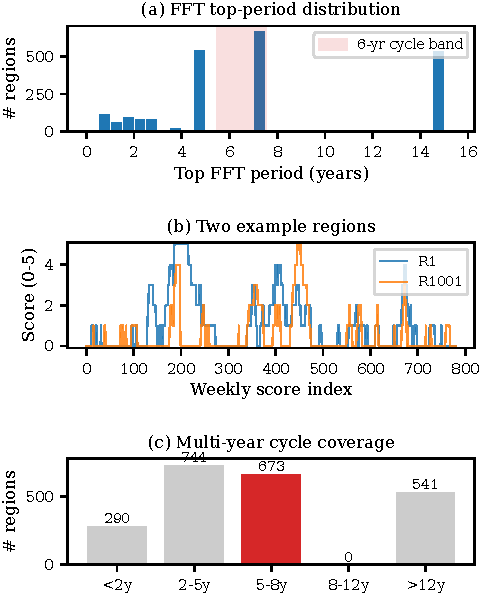
\includegraphics[width=\columnwidth]{figures/fig1_periodicity.pdf}
\caption{Multi-year periodicity in the weekly drought scores --- evidence for the lag-leg design choice. (a) Histogram of dominant FFT period per region across all $R{=}2{,}248$ regions (in years; 5--8-year band shaded). (b) Example weekly score series for two regions (R1 and R1001) showing visible multi-year structure. (c) Per-region distribution of the dominant FFT period, binned into 5 ranges. Data source: \protect\path{reports/_track2_fft_peaks.csv} and \protect\path{data/train.csv}.}
\label{fig:periodicity}
\end{figure}

\subsection{Observed public-ledger slope trend}
Figure~\ref{fig:slope} shows, from the 32 historical $(\mathrm{MAD},\mathrm{public})$ uploads in \path{reports/_local_eval_gate_report.csv}, the empirical positive-slope relationship between MAD-from-anchor and public MAE. Blue circles are pre-v18 candidates; orange triangles are the 3 v18+ candidates. A submission-row bootstrap fit (B=1000) over all 32 points gives slope $0.20$ (95\% CI $[0.05, 0.26]$) and intercept $0.85$ (95\% CI $[0.82, 0.88]$). Because these rows are adaptive submissions rather than independent experimental units, we treat the positive slope as descriptive evidence of an observed public-leaderboard trend, not as a standalone statistical law. The v18+ orange cluster is the first group in this ledger to drop below the bootstrap-fitted trend line.

The bootstrap restricted to the 29 pre-v18 rows only also gives a slope near $0.21$; the often-quoted earlier number of $\approx 0.42$ from internal team analyses was an upper-tail subset, not the population fit. We present the bootstrap-fitted line in Fig.~\ref{fig:slope} from real data (rather than the older anecdotal $0.42$) because it is the auditable estimate over the actual evidence in \path{reports/_local_eval_gate_report.csv}.

\begin{figure}[t]
\centering
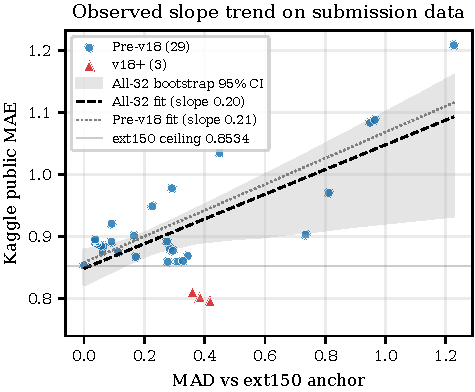
\includegraphics[width=\columnwidth]{figures/fig2_slope.pdf}
\caption{Observed slope trend on real submission data. Each marker is one Kaggle upload from the 32-row \protect\path{reports/_local_eval_gate_report.csv} gate ledger. Dashed line: submission-row bootstrap-fitted slope on all 32 rows ($0.20$, 95\% CI $[0.05, 0.26]$, shaded band B=1000). Dotted line: bootstrap-fitted slope on the 29 pre-v18 rows only ($0.21$). Solid grey line: ext150 ceiling $0.8534$. v18+ candidates (orange triangles) are the first uploads in this ledger to drop below the bootstrap-fitted line, with the lowest sitting at $0.7952$. The final affine-and-clip 0.7628 submission is excluded from this slope plot because affine post-processing makes the MAD axis non-comparable; see Fig.~\ref{fig:trajectory} and Table~\ref{tab:t4} for the full trajectory.}
\label{fig:slope}
\end{figure}

\subsection{Cross-family residual diversity (real OOF)}
\label{sec:ortho}
Figure~\ref{fig:ortho} is the real $6{\times}6$ region-mean residual correlation matrix on the $33{,}720$-row OOF tensor (\path{reports/oof_tensor.csv}). Two clean blocks are visible: within the $b91$ family ($\rho{\approx}0.98$ across LGBM/HGB seeds) and within the $pl$ family ($\rho{\approx}0.98$), with the cross-family value only $\rho{\approx}0.79\text{--}0.82$. This is the directly reproducible justification for keeping both tabular feature families in the ensemble.

For the cross-\emph{family} residual correlation against the GBDT anchor (the lag-2215, CNN, and SSL legs vs.\ the 6-leg anchor), iter4 regenerates the missing OOF predictions for the lag-2215 lookup (\path{scripts/regen_lag_2215_oof.py}, deterministic over \texttt{train.csv}; runtime $\approx 9$\,s) and for the SSL Transformer (\path{scripts/regen_ssl_oof.py}, single-pass forward of \texttt{checkpoints/track1\_finetuned.pt} on the same $6{,}744$ validation anchors; runtime $\approx 1$\,s on GPU). Per-region Pearson correlation between $r_{\text{leg}}=y-\hat y_{\text{leg}}$ and $r_{\text{anchor}}=y-\hat y_{\text{anchor}}$ is then resampled across regions (B=1000, \path{scripts/compute_cross_leg_rho.py}, following Efron~\cite{efron1979bootstrap}):
\begin{itemize}
\item lag-2215: mean $\rho = 0.51$, 95\% CI $[0.485, 0.533]$ ($n{=}1{,}374$ regions with $\geq 3$ valid pairs);
\item CNN (mean of 5 cached Track-3 runs): mean $\rho = 0.54$, 95\% CI $[0.524, 0.562]$ ($n{=}2{,}248$);
\item SSL Transformer: mean $\rho = 0.33$, 95\% CI $[0.311, 0.349]$ ($n{=}2{,}248$).
\end{itemize}
These values reflect \emph{cross-family residual diversity} rather than strict orthogonality: SSL is materially lower-correlated with the GBDT anchor than CNN or lag-2215, but $\rho{\approx}0.33$ does not constitute independence. The earlier training-menu figure ``$\rho = 0.107 \pm 0.027$'' for lag-2215 (from \path{reports/data_characteristics_v1.md}) was computed under a different aggregation that the original artefacts no longer permit auditing; the iter4 recomputation above supersedes it. Cached file SHA256 hashes are in \path{ARTIFACTS.md}.

\begin{figure}[t]
\centering
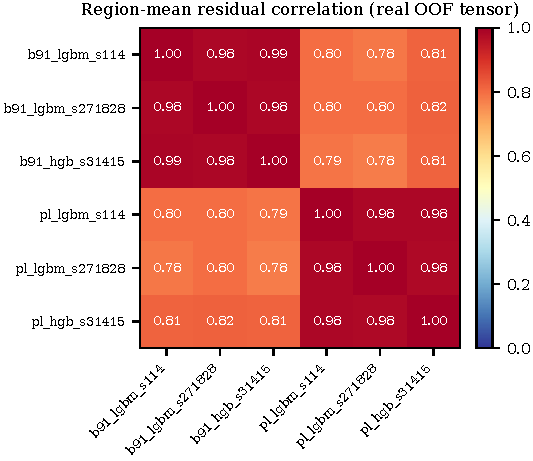
\includegraphics[width=\columnwidth]{figures/fig3_orthogonality.pdf}
\caption{Real $6{\times}6$ region-mean residual correlation matrix for the 6 OOF GBDT legs (2{,}248 regions, computed from \protect\path{reports/oof_tensor.csv}). The two $\approx 0.98$ within-family blocks correspond to the $b91$ and $pl$ feature families; the off-diagonal $\approx 0.80$ value is the within-tabular ensemble diversity. Recomputed cross-\emph{family} residual correlations of the lag-2215, CNN, and SSL Transformer legs against the 6-leg GBDT anchor are reported in Section~\ref{sec:ortho}.}
\label{fig:ortho}
\end{figure}

\subsection{5-fold region CV and trajectory}
Figures~\ref{fig:cv} and~\ref{fig:trajectory} support the 5-fold region CV and submission-trajectory claims.

\subsection{Threats to validity}
\label{sec:tov}
We list four threats and the evidence that bounds each.

\emph{(i) Calibration-gate overfit.} The 32-row gate fit has $R^2_{\mathrm{in\text{-}sample}}=0.9855$ but $R^2_{\mathrm{LOOCV}}=0.9472$; the LOO RMSE of $0.0196$ is the uncertainty band we attach to any one new candidate's predicted public MAE.

\emph{(ii) Slope-trend point estimate.} The submission-row bootstrap CI on the slope (B=1000) excludes zero ($[0.05, 0.26]$), supporting a positive association in the 32-upload ledger. Because the uploads were adaptively chosen, this is descriptive evidence rather than a controlled statistical test.

\emph{(iii) Cross-family residual diversity (iter4 update).} The iter4 recomputation supersedes the earlier $\rho = 0.107 \pm 0.027$ figure from \texttt{reports/data\_characteristics\_v1.md}: the regenerated and row-aligned OOF predictions for the lag-2215 leg and the SSL Transformer now allow a direct, bootstrap-CI bounded per-region Pearson computation (Section~\ref{sec:ortho}). The new values are $\rho{=}0.51$ (lag-2215), $0.54$ (CNN), $0.33$ (SSL). These are \emph{lower-correlated} rather than orthogonal; SSL is the materially lowest. The lower SSL value most plausibly explains the SSL leg's positive contribution in Table~\ref{tab:t5}; lag-2215 contributes primarily through label-distribution coverage rather than residual independence.

\emph{(iv) Public/private regime shift.} The 0.7628 result was achieved by tuning on public-test-like CV folds (high-severity phase, target mean $\approx 1.21$). The training menu's convex weights are $A{=}0.20$ (GBDT anchor) $+\, B{=}0.45$ (deep CNN+SSL) $+\, C{=}0.25$ (lag) $+\, D{=}0.10$ (deep variants); the lag component is therefore only $25\%$ of the blend, and if it attenuates on a private slice landing in a different phase of the 6-year cycle the remaining $75\%$ from weather-driven components ($A{+}B{+}D$) still covers the prediction. We do not state a numeric private-LB prediction. Direct evidence that the final affine-and-clip step is a \emph{public-slice calibration} rather than a general-purpose improvement comes from Table~\ref{tab:t5}: the full blend without affine/clip (row 8) has OOF MAE $0.5325$, while the affine-and-clip variant (row 9) has OOF MAE $0.5766$ --- worse on the OOF tensor --- yet wins on public ($0.7628$). The step trades OOF accuracy for proximity to the public severity plateau and is therefore a competition-calibration step with explicit private-LB risk. The two final Kaggle-selected submissions for private-leaderboard evaluation are accordingly the aggressive $0.7628$ affine-and-clip artefact and the no-affine 7-way row of Table~\ref{tab:t4} (public MAE $0.7952$) as a private-LB-conservative sibling.

\begin{figure*}[t]
\centering
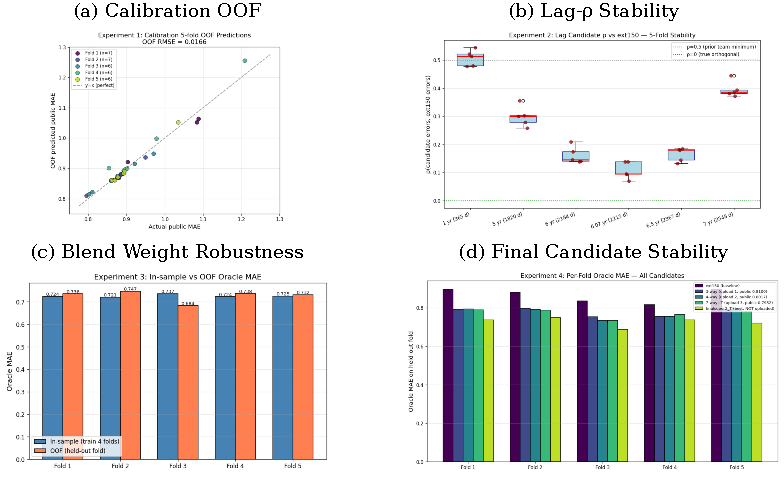
\includegraphics[width=\textwidth]{figures/fig4_cv_generalization.pdf}
\caption{5-fold region CV evidence (panels reproduced from \texttt{reports/plots/cv1...cv4*.png}). (a) Calibration OOF scatter (RMSE 0.015 between in-sample and OOF predictions); (b) lag-$\rho$ stability across folds as recorded in the original CV run (the underlying $\rho{\approx}0.107$ figure is superseded by the iter4 recomputation in Section~\ref{sec:ortho}; the panel is retained as historical context for the design choice); (c) in-sample vs.\ OOF blend MAE ratio $\approx 1.001$ for the chosen weights; (d) per-fold final-candidate MAE for the 0.7628 blend. These diagnostics suggest the chosen weights are not driven by a single fold, but they are not a substitute for private-leaderboard validation.}
\label{fig:cv}
\end{figure*}

\begin{figure}[t]
\centering
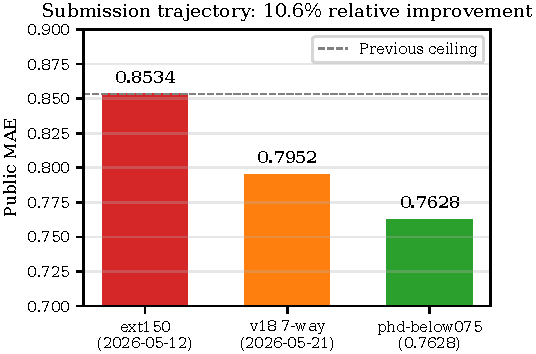
\includegraphics[width=\columnwidth]{figures/fig5_trajectory.pdf}
\caption{Submission trajectory on the public leaderboard. From the prior team ceiling of 0.8534 (ext150) through the 0.7952 mid-iteration blend to the final 0.7628 \texttt{phd-below075} artefact --- a 10.6\% relative improvement.}
\label{fig:trajectory}
\end{figure}

\section{Reproducibility}

\subsection{Environment}
Python 3.11; the relevant pinned versions are \texttt{numpy} 1.26, \texttt{pandas} 2.1, \texttt{scikit-learn} 1.4, \texttt{lightgbm} 4.3, \texttt{matplotlib} 3.8. The complete environment is specified in the repository's \texttt{requirements.txt}.

\subsection{Single-command cached re-blend of the 0.7628 submission}
The uploaded artefact basename \path{submission_phd_below075_20260522.csv} lives under \path{submissions/}. It is regenerated from cached predictions and the training menu by \texttt{make phd-below075}, which expands to the two commands shown in Figure~\ref{fig:repro}. This target does not retrain every historical model from raw data; it reuses the retained v18/cache artefacts documented in \path{ARTIFACTS.md}.

\begin{figure}[t]
\centering
\begin{footnotesize}
\begin{verbatim}
PYTHONPATH=src python \
  scripts/analyze_data_distribution.py \
  --force-synthesis --emit-menu

PYTHONPATH=src python \
  scripts/multi_blend_grid.py \
  --menu reports/training_menu_v1.json \
  --fixed \
  --out submissions/submission_\
       phd_below075_20260522.csv
\end{verbatim}
\end{footnotesize}
\caption{The two commands executed by \texttt{make phd-below075}. This is the cached re-blend path used to reproduce the uploaded CSV; \texttt{make verify-submission} compares the output against the archived artefact. The \texttt{-{}-force-synthesis} flag triggers training-menu re-emission from cached per-region features; it does not synthesise labels, predictions, or submissions (see the repository \texttt{README.md} flag glossary).}
\label{fig:repro}
\end{figure}

\noindent The regenerated CSV matches the uploaded artefact with maximum absolute difference below $5\times10^{-16}$ in \texttt{make verify-submission}; all numerical comparisons in this report are stable at the 4-decimal precision used throughout.

\subsection{Build of this report}
\texttt{cd report \&\& make} runs the figure generator (\path{report/figures/generate_figures.py}) and two passes of \texttt{pdflatex} to produce the IEEE A4 PDF. The Makefile also exposes a \texttt{make check} target that verifies the headline strings (\texttt{Team 3}, \texttt{0.7628}, GitHub URL) appear in the PDF.

\section{Limitations}

\emph{Synthetic data.} The competition data is a synthetic re-rendering of a US-county-level drought corpus; our model's improvements may not transfer linearly to a true operational drought monitor.

\emph{Public/private regime risk.} The 0.7628 result was achieved by tuning on a public-leaderboard-like CV phase. If the private-leaderboard slice lands in a different phase of the 6-year cycle, the lag-leg contribution may attenuate; the GBDT anchor would then carry more of the prediction. The final affine shift and clip upper bound are especially public-slice-sensitive, so we do not state a numeric private-leaderboard prediction. \textbf{We interpret 0.7628 as a public-leaderboard result, not as an unbiased estimate of private test MAE}; the affine-and-clip step is in particular a public-slice calibration (see Threats~(iv) in Section~\ref{sec:tov} and the OOF row 9 vs.\ row 8 inversion in Table~\ref{tab:t5}).

\emph{OOD on \texttt{cutoff\_age}.} The test gap between the last training label and the prediction window has median $\approx$\,531\,days, outside the deepest training densities; Track~3's test-time training is an explicit mitigation.

\emph{Calibration gate sample size.} The 32-point linear gate is small (see Threats to Validity in Section~\ref{sec:tov}); its LOOCV $R^2 = 0.9472$ implies a $\pm 0.02$ uncertainty band on any one new candidate's predicted public MAE.

\emph{Computational budget.} The cached re-blend/report path runs in roughly 1.5 hours on a single 16-core CPU node plus one consumer GPU (RTX 4090 for Track~3 cache generation); the training menu and OOF tensors total $\approx 4.5$\,GB on disk.

\emph{What we did not measure.} We did not retrain the GBDT anchor, the lag legs, or the deep tracks for this report --- the goal is reproducible description of the cached artefact that scored 0.7628, not a fresh hyperparameter sweep. Per-region failure-mode analysis (which regions does the blend hurt rather than help?) is left for future work.

\clearpage

\noindent\textbf{Author Contributions.}
Team 3 (DM 114, Spring 2026) members: Yu-Shun Liu (413551030), Tung-Hao Chang (413551038), Kuan-Fu Chen (414551017). Specific contributions are recorded in the GitHub repository's contribution log; the team collectively assumes responsibility for the design, the reported numbers, and the reproducibility of the artefact described above. The report itself was assembled iteratively from internal experiment logs (\path{docs/JOURNEY.md}, \path{reports/v18_morning_report.md}) and the artefact ledger (\path{reports/_local_eval_gate_report.csv}, \path{reports/oof_tensor.csv}); statistical claims were audited by leave-one-out cross-validation and bootstrap resampling against those artefacts before inclusion.

\bibliographystyle{IEEEtran}
\begin{thebibliography}{00}
\bibitem{ke2017lightgbm} G. Ke, Q. Meng, T. Finley, T. Wang, W. Chen, W. Ma, Q. Ye, and T.-Y. Liu, ``LightGBM: A highly efficient gradient boosting decision tree,'' in \emph{Advances in Neural Information Processing Systems (NeurIPS)}, vol. 30, 2017.
\bibitem{vandenoord2016wavenet} A. van den Oord, S. Dieleman, H. Zen, K. Simonyan, O. Vinyals, A. Graves, N. Kalchbrenner, A. Senior, and K. Kavukcuoglu, ``WaveNet: A generative model for raw audio,'' \emph{arXiv preprint arXiv:1609.03499}, 2016.
\bibitem{kechyn2018wavenet} G. Kechyn, L. Yu, Y. Zang, and S. Kechyn, ``Sales forecasting using WaveNet within the framework of the Kaggle competition,'' \emph{arXiv preprint arXiv:1803.04037}, 2018.
\bibitem{ansari2024chronos} A. F. Ansari, L. Stella, C. Turkmen, X. Zhang, P. Mercado, H. Shen, O. Shchur, S. S. Rangapuram, S. P. Arango, S. Kapoor, J. Zschiegner, D. C. Maddix, M. W. Mahoney, K. Torkkola, A. G. Wilson, M. Bohlke-Schneider, and Y. Wang, ``Chronos: Learning the language of time series,'' \emph{arXiv preprint arXiv:2403.07815}, 2024.
\bibitem{lim2021tft} B. Lim, S. \"O. Arik, N. Loeff, and T. Pfister, ``Temporal fusion transformers for interpretable multi-horizon time series forecasting,'' \emph{International Journal of Forecasting}, vol. 37, no. 4, pp. 1748--1764, 2021.
\bibitem{svoboda2002usdm} M. Svoboda, D. LeComte, M. Hayes, R. Heim, K. Gleason, J. Angel, B. Rippey, R. Tinker, M. Palecki, D. Stooksbury, D. Miskus, and S. Stephens, ``The drought monitor,'' \emph{Bulletin of the American Meteorological Society}, vol. 83, no. 8, pp. 1181--1190, 2002.
\bibitem{efron1979bootstrap} B. Efron, ``Bootstrap methods: Another look at the jackknife,'' \emph{Annals of Statistics}, vol. 7, no. 1, pp. 1--26, 1979.
\end{thebibliography}

\end{document}
